% !TeX spellcheck = pl_PL
\documentclass[a4paper,twoside]{article}
\usepackage{polski}
\usepackage[utf8]{inputenc}
\usepackage{graphicx}
\usepackage{amsmath}

\usepackage[unicode, bookmarks=true]{hyperref} %do zakładek
\usepackage{tabto} % do tabulacji
\NumTabs{6} % globalne ustawienie wielkosci tabulacji
\usepackage{array}
\usepackage{multirow}
\usepackage{array}
\usepackage{dcolumn}
\usepackage{bigstrut}
\usepackage{color}
\usepackage[usenames,dvipsnames]{xcolor}
\usepackage{svg}
\usepackage{xfrac}
\usepackage{floatrow}
\usepackage{enumitem}

\usepackage{multirow,tabularx}
\newcolumntype{Y}{>{\centering\arraybackslash}X}
\renewcommand{\arraystretch}{2}

% === Reset inkrementacji sekcji przy nowym parcie === %
\usepackage{titlesec}

\makeatletter
\@addtoreset{section}{part}
\makeatother
\titleformat{\part}[display]
{\normalfont\LARGE\bfseries\centering}{}{-60pt}{}

% === Dodanie krpki do sekcji
\titlelabel{\thetitle.\quad}


\setlength{\textheight}{24cm}
\setlength{\textwidth}{15.92cm}
\setlength{\footskip}{10mm}
\setlength{\oddsidemargin}{0mm}
\setlength{\evensidemargin}{0mm}
\setlength{\topmargin}{0mm}
\setlength{\headsep}{5mm}

\setlength{\textfloatsep}{10pt plus 1.0pt minus 2.0pt}


\begin{document}
	\bibliographystyle{plain}
	
	% ************************************************************
	% --- Strona tytułowa
	% ************************************************************
	\begin{titlepage}
		\begin{table}[htbp]
			\centering
			\begin{tabular}{|c|c|c|c|c|c|c|}
				\hline
				\multicolumn{7}{|c|}{\textbf{{\LARGE Grafika Komputerowa}}} \bigstrut\\[4pt]
				\hline
				Rok akademicki & Termin & Rodzaj studiów & Kierunek & Prowadzący & Grupa & Sekcja \bigstrut\\
				\hline
				\multicolumn{1}{|c|}{\multirow{2}[4]{*}{{\large 2014/2015}}} & \multicolumn{1}{c|}{{\large Wtorek}} & \multicolumn{1}{c|}{\multirow{2}[4]{*}{{\large SSI}}} & \multicolumn{1}{c|}{\multirow{2}[4]{*}{{\large INF}}} & \multicolumn{1}{c|}{\multirow{2}[4]{*}{\begin{tabular}{@{}c@{}}{\large dr} \\[-9pt] {\large Ewa Lach}\end{tabular}}} & \multicolumn{1}{c|}{\multirow{2}[4]{*}{{\large GKiO3}}} & \multicolumn{1}{c|}{\multirow{2}[4]{*}{{\large 1}}} \bigstrut\\
				\cline{2-2}    \multicolumn{1}{|c|}{} & \multicolumn{1}{c|}{{\large 12:45 - 15:00}} & \multicolumn{1}{c|}{} & \multicolumn{1}{c|}{} & \multicolumn{1}{c|}{} & \multicolumn{1}{c|}{} & \multicolumn{1}{c|}{} \bigstrut\\
				\hline
			\end{tabular}%
		\end{table}%
		
		\centering
		\includegraphics[width=0.6\textwidth]{./images/logo.png}
		\\\vspace{10mm}
		\textbf{{\huge Karta projektu}}\\\vspace{5mm}
		\textbf{{\Huge Danmaku Shooter}}
		\\
		\vfill
		\begin{flushright}
			{\Large \textbf{Skład sekcji}:}\\
			\begin{tabular}{rr}
				{\Large Buchała} & {\Large Bartłomiej}\\[-3pt]
				{\Large Forczmański} & {\Large Mateusz}\\[-3pt]
				{\Large Motyka} & {\Large Marek}\\[-3pt]
				{\Large Wudecki} & {\Large Wojciech}
			\end{tabular}
		\end{flushright}
		
	\end{titlepage}
	
	
	
	% ************************************************************
	% --- Strona z założeniami
	% ************************************************************
	\part{\huge \textbf{Krótki opis aplikacji}}
		\textit{Shoot' em up} (w skrócie zwany shmup) jest gatunkiem gier akcji wywodzącym się w prostej linii od gier typu \textit{Space Invaders} lub \textit{River Raid}. Kontrolowana przez gracza postać (np. statek) w pojedynkę stawia czoło przeciwnikom, niszcząc ich za pomocą wystrzeliwanych pocisków, jednocześnie unikając ich ataków. Podgatunek shmupów, zwany \textit{danmaku} (z jap. \textit{ściana pocisków} lub \textit{piekło pocisków}) kładzie większy nacisk na omijanie wrogich ataków, niż na ofensywie. Przykładowymi danmaku są np. \textit{Ikaruga} czy większość gier z uniwersum \textit{Touhou Project}. \\
	
		Gra powstawać będzie jako projekt łączony z przedmiotów Projekt Programistyczny i Grafika Komputerowa.
	
	\begin{center}
		\fbox{%
			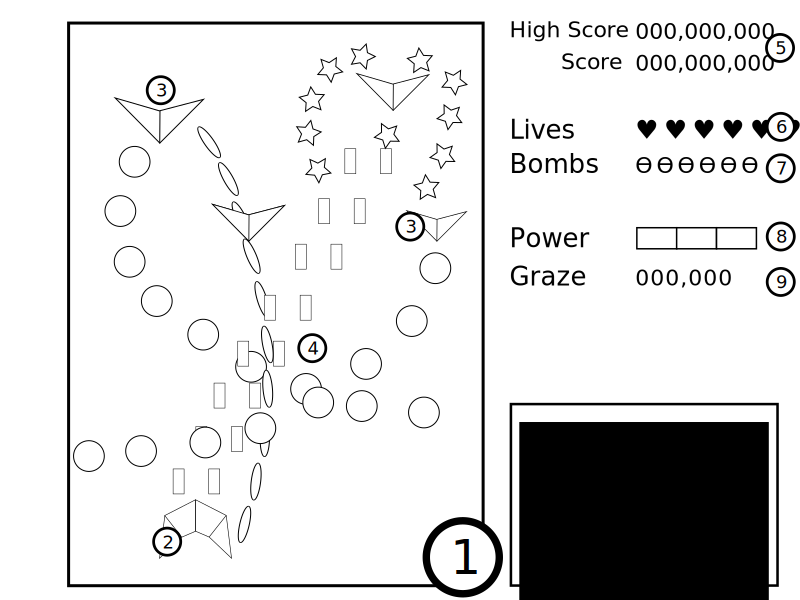
\includegraphics[width=0.8\textwidth]{./images/screen01}%
		}
		\vspace{5pt}
	\end{center}
	\begin{enumerate}
		\item Ekran gry właściwej. W jej obrębie znajduje się gracz, pociski oraz wszyscy wrogowie. 
		\item Grywalna postać, porusza się po ekranie gry, unikając pocisków oraz strzelając do wrogów.
		\item Wrogowie, których należy pokonać.
		\item Chmara pocisków. Jak widać na rysunku, nie wchodzą ze sobą w żadną interakcję, każdy leci swoim wyznaczonym torem. Sprajty wrogów są niewrażliwe na swoje pociski, nie występuje \textit{friendly fire}.
		\item Liczba zdobytych punktów oraz porównywanie ich z największym wynikiem.
		\item Liczba pozostałych żyć. W trakcie gry można zdobywać kolejne. Utrata wszystkich kończy grę.
		\item Liczba pozostałych bomb. Każda wykorzystana bomba zapewnia kilkusekundową odporność na wrogie pociski oraz umożliwia pojedynczy silniejszy atak. Można je zdobyć w trakcie gry.
		\item Pasek mocy, napełnia się w trakcie gry wraz ze zdobytymi punktami. Utrata życia skutkuje zmniejszeniem paska o 1 segment.
		\item Liczba "otarć", czyli uniknięć bardzo blisko pocisku. Aby umożliwić większe wyzwanie, ostateczny wynik pomnożony jest przez licznik Graze.
	\end{enumerate}
	
	
	\newpage
	
	\part{\huge \textbf{Analiza zadania}}
	
	\section{Podstawy teoretyczne problemu}
		\subsection{Przestrzeń fizyczna}
			W naszej grze w interakcję ze sobą będzie wchodzić bardzo dużo elementów, począwszy od gracza, a na ostatnim z setki pocisków skończywszy. Bardzo ważne jest, aby ruchy i interakcje wszystkich elementów były ze sobą zsynchronizowane, a droga o długości 1 była tym samym dla każdego z nich.\\
			W tym celu zdecydowaliśmy się na wprowadzenie do gry przestrzeni fizycznej, w której będą zachodzić wybrane przez nas zjawiska fizyczne, potrzebne dla realizacji gry.
			
		\subsection{Ruch}
			Każdy obiekt, który może się poruszać i zmienić swoje położenia, posiada swoją prędkość. W naszej grze wyróżniliśmy 3 rodzaje ruchu:
			\subsubsection{Ruch jednostajny}
				W jednostce czasu ciało pokonuje jednakową drogę, a przebyta droga jest proporcjonalna do czasu.
				$$ v=\cfrac{s}{t}=const$$
				Gdzie $ v $ to prędkość, $ s $ - droga, a $ t $ to czas. W naszym obiekty poruszają się na ekranie, więc jednostką długości jest piksel.
			\subsubsection{Ruch jednostajnie przyspieszony}
				W jednostce czasu prędkość ciała ulega zwiększeniu o stałą wartość.
				$$ v(t)=v_0+a\cdot t $$
			\subsubsection{Ruch jednostajnie opóźniony}
				W jednostce czasu prędkość ciała ulega pomniejszeniu o stałą wartość.
				$$ v(t)=v_0-a\cdot t $$
			
		
		\newpage
		\subsection{Tor pocisków}
			Jednym z podstawowych problemów w naszym zadaniu jest tor po jakim poruszają się pociski. Obiekty wrogów będą poruszać się w prosty sposób, jednak zbiory pocisków będą układać się w skomplikowane wzory, tworzyć ze sobą specyficzny układ. W naszej grze chcemy zaimplementować pociski, które będą poruszać się m.in. po takich torach jak okrąg i elipsa.\\
		
		\subsubsection{Okrąg}
			Wybraliśmy opis w postaci równania parametrycznego, który jest wygodniejszy i bardziej efektywny w implementacji:
			$$
				\begin{cases}
					x=x_0+r\cdot \cos{\alpha}\\
					y=y_0+r\cdot \sin{\alpha}
				\end{cases}
			$$
			Gdzie punkt $ O(x_0, y_0) $ jest środkiem okręgu, $ r $ promieniem, a parametr $ \alpha \in [0, 2\pi ) $.
		\subsubsection{Elipsa}
			Podobnie jak wyżej, elipsę zdefiniowaliśmy równaniem parametrycznym:
			$$
				\begin{cases}
					x=x_0+a\cdot \cos{\alpha}\\
					y=y_0+b\cdot \sin{\alpha}
				\end{cases}
			$$
			Gdzie punkt $ O(x_0, y_0) $ jest środkiem elipsy, $ a,\:b $ długościami półosi, a parametr $ \alpha \in [0, 2\pi ) $.
		\subsubsection{Spirala}
			Tor spirali jest zdefiniowany równaniem parametrycznym:
			$$
				\begin{cases}
					x=x_0+a\cdot \alpha \cos{\alpha}\\
					y=y_0+b\cdot \alpha \sin{\alpha}
				\end{cases}
			$$
			Gdzie punkt $ O(x_0, y_0) $ jest punktem centralnym spirali, $ a,\:b $ długościami półosi, a parametr $ \alpha \in [0, \inf ) $.
		
	\newpage
	\section{Wykorzystywane zagadnienia grafiki komputerowej}
		\subsection{Przekształcenia afiniczne}
			Postanowiliśmy wykorzystać na poznane na laboratorium przekształcenia afiniczne. Wszystkie ruchome obiekty w naszej grze, które zmieniają dynamicznie swoją pozycję, będą korzystać z trzech wybranych przekształceń:
			\subsubsection{Translacja}
				Przesunięcie punktu $ P=(x, y, z) $ o wektor $ d=[d_x, d_y, d_z] $, w wyniku którego powstaje obraz\\ $ P=(x', y', z') $, gdzie:
				$$
					\begin{cases}
						x'=x+d_x\\
						y'=y+d_y\\
						z'=z+d_z
					\end{cases}
				$$
			\subsection{Skalowanie}
				W naszym programie wszystkie przekształcenia skalowania będą zachowywać proporcje, więc zdefiniować je jako: przesunięcie punktu $ P=(x, y, z) $ o współczynnik skalowania $ s $, w wyniku którego powstaje obraz\\ $ P=(x', y', z') $, gdzie:
				$$
					\begin{cases}
						x'=s\cdot x\\
						y'=s\cdot y\\
						z'=s\cdot z
					\end{cases}
				$$
			\subsection{Obrót}
				
	
	\section{Wykorzystywane biblioteki i narzędzia programistyczne}
		\subsection{DirectX 9}
			Jako narzędzie do budowania obiektów graficznych zdecydowaliśmy się na DirectX w wersji 9. Jako alternatywne rozwiązanie rozważaliśmy DirectX 11, jednak nasza gra będzie budowana na scenie 2D, a DirectX 9 oferuje wygodniejsze narzędzia - wciąż operuje na takich klasach jak Sprite lub Texture, które są lepsze dla naszej gry. DirectX 11 wszystkie te klasy zastępuje interfejsem IResource, który wymaga odpowiedniej konwersji (większe nastawienie na grafikę trójwymiarową). By móc wykorzystać DirectX 11 do pracy na zwykłych sprajtach, wymagane byłyby dodatkowe zestawy narzędzi, jak np. DirectX Tool Kit.\\
			Jako konkurencyjne rozwiązanie dla samego DirectXa rozważaliśmy OpenGL, jednak nasz program będzie zorientowany obiektowo, a DirectX daje lepsze możliwości enkapsulacji.\\
			Ponadto, dzięki DirectXowi wygodniejsze jest pracowanie m.in. z przekształceniami afinicznymi modeli 3D.
			% Czuję się jak prawdziwy Windziarz // Forczu-sama
		\subsection{Microsoft Visual Studio 2012}
			
		\subsection{Enterprise Architect}
			Jako narzędzie do zaprojektowania gry w modelu zorientowanym obiektowo wybraliśmy Enterprise Architect. Głównym powodem była nasza znajomość języka UML, którego uczymy się na studiach od ponad roku, a także doświadczenie z tym środowiskiem. Zdecydowaną zaletą wcześniejszego zaprojektowania aplikacji w tym środowisku jest wygoda obsługi, łatwość tworzenia diagramów oraz możliwość generacji kodu. Samo zdecydowanie się na wcześniejsze utworzenie diagramów UML umożliwi nam lepszą kontrolę nad pracą oraz zapewnienie wszystkich potrzebnych możliwości naszej aplikacji.
	
	
	\section{Algorytmy, struktury danych, ograniczenia specyfikacji}
	
	\newpage
	
	\part{Plan pracy}
		\section{Zaprojektowanie gry w języku UML}
			\begin{enumerate}[label=\alph*.]
				\item Utworzenie modelu przypadków użycia aktora Gracza
				\item Utworzenie modelu klas, w postaci diagramu, z wszystkimi potrzebnymi relacjami.
				\item Zarysowanie scenariuszy pierwszoplanowych.
			\end{enumerate}
		\section{Przygotowanie szkieletu aplikacji}
			\begin{enumerate}[label=\alph*.]
				\item Napisanie okna w WIN API jako punktu wejściowego aplikacji.
				\item Inicjalizacja silnika graficznego Direct 3D w celu umożliwienie pisania i testowania obiektów graficznych od samego początku.
				\item Zdefiniowanie zegara gry, do którego obiektu muszą dostosowywać swoje zachowanie.
				\item Napisanie klasy nadrzędnej GameObject dla ruchomych obiektów gry - podstawa dla przekształceń afinicznych.
				\item Klasa Sprite służąca do rysowania i kontroli elementów gry. W późniejszej części pracy, dopóki modele sprajtów końcowych nie będą gotowe, będziemy pracować na prymitywach.
			\end{enumerate}
		\section{Części niezależne od siebie}
			\begin{enumerate}[label=\alph*.]
				\item Implementacja klasy Gracza, synchronizacja z klawiaturą, umożliwienie strzelania i wykorzystywania bomb.
				\item Napisanie klasy Pocisk oraz Wzorzec, które kontrolują pociski i układają je we układy oparte na wzorach matematycznych
				\item Napisanie klas Wrogów oraz integracja ich z typem wrogich pocisków
				\item Utworzenie ekranu powitalnego (tzw. \emph{title screen}) umożliwiającego zmianę konfiguracji i rozpoczęcie gry.
				\item Stworzenie uniwersalnej konfiguracji klawiszy - zdefiniowanie kontrolek dla Gracza oraz możliwości ich zmiany przez użytkownika.
			\end{enumerate}
		\section{Części zależne od siebie}
			\begin{enumerate}[label=\alph*.]
				\item Umożliwienie interakcji Hitboxów - implementacja otarć, kolizji, straty życia.
				\item Szczegółowa integracja obiektów gry na scenie: określenie w których momentach pojawiają się wrogowie, kiedy strzelają, kiedy zostają wyeliminowani.
				\item Naliczanie zdobytych punktów
			\end{enumerate}
		\section{Wykonanie modeli graficznych}
			\begin{enumerate}[label=\alph*.]
				\item Narysowanie obiektu statku w technice 3D.
				\item Narysowanie tła ekranu powitalnego oraz gry, a także panelu ze statystyką.
				\item Narysowanie modeli wrogów.
				\item Narysowanie kształtów pocisków oraz bonusów, opartych o prymitywy.
			\end{enumerate}
		
	
	\newpage
	
	\part{Podział pracy}
		% --- Słowem wstępu
		Jako podstawową metodę podziału pracy wybraliśmy oddzielnie pisanie klas programu. Zaczynamy od wspólnego napisania klas wymaganych w sekcji [Przygotowanie szkieletu aplikacji], a następnie każdy przechodzi do niezależnego wykonania pozostałej części swoich zadań. Gdy nadejdzie taka konieczność, klasy będą ze sobą odpowiednio zsynchronizowane.
	
	
\end{document}